\documentclass[10pt,a4paper]{article}
\usepackage[latin1]{inputenc}
\usepackage{amsmath}
\usepackage{float}
\usepackage{graphicx}
\usepackage{fullpage}
\usepackage{caption}

\begin{document}
\captionsetup{width=0.8\textwidth}

\author{Jeroen Hofman\\
  		10194754\\
		}
\title{Stochastic Simulation Project 1\\
       Integrating the Mandelbrot set
		}
\maketitle

\newpage

\section{Introduction}
In this report we use stochastic simulations to integrate the Mandelbrot set. We first describe the definition of the Mandelbrot set. Next we describe which methods we used to calculate the integral. In the results section the results from this method are shown. The discussion at the end gives some points of improvement. 

\section{Theory}
\noindent The Mandelbrot set is a so called \emph{fractal}, which is a geometric shape with a high amount of self-similarity, i.e. by zooming in on a part of the fractal a partial copy of the fractal is obtained. Fractals can be defined by recurrence formulas, and the Mandelbrot set is an interesting fractal because its exact area is not known. There are however many computational studies which have tried to determine the area of the set. A study by reference \cite{paper1} has computed the area of a Mandelbrot set by using a technique called pixel counting. Pixel counting is a technique where the Mandelbrot set is generated on a grid and the area of the set can be estimated by counting the number of pixels that are in the set after a large number of iterations (defined below). The best known value for the Mandelbrot set is $1.506 591 77 \pm 0.000 000 08$.
\newline
\newline
\noindent The Mandelbrot set is generated using the following (complex-valued) equation:\\
\begin{equation}
P_{c}: z \mapsto z^{2} + c  
\end{equation}
\noindent where a point $c$ in the complex plane is in the Mandelbrot set if and only if:\\
\begin{equation}
\label{eq:eq1}
|P^{n}_{c}(0)| \leq 2 \; \text{for all} \; n > 0
\end{equation}
\noindent Since this condition has to hold for all $n$ and has to be computed for the whole complex plane, the area of the Mandelbrot set cannot be solved exactly by a computer. Below is a simple graph showing the Mandelbrot set for the first 100 iterations, where the points that are computed are on an equally spaced grid of size 1000x1000.

\begin{figure}[H]
  \centering
  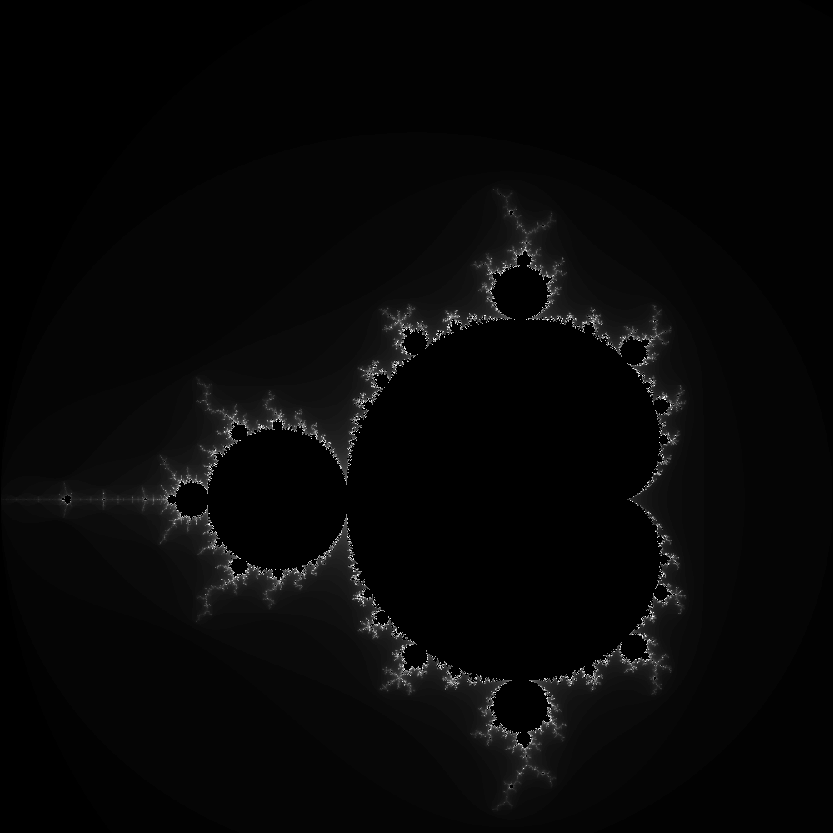
\includegraphics[scale=0.6]{mandelbrot.pdf}
  \caption{Visualization of the Mandelbrot set on the complex plane obtained by computing the condition in equation \ref{eq:eq1} for $n \leq 100$ for points in the complex plane equally spaced on a grid of size 1000x1000.}
  \label{fig:mandelbrot}
\end{figure}

\section{Methods}

\noindent Apart from the method of pixel counting one can also use sampling to estimate the area of the Mandelbrot set. By sampling one considers a random point in the complex plane and computes whether or not this point is in the Mandelbrot set by using the condition in equation \ref{eq:eq1} for some maximum iteration depending on the computer power. By repeating this and taking many random sample points the area of the set can be estimated by dividing the amount of samples in the set by the total amount of samples $N_{\text{samples}}$, and multiplying this by the total area on which the samples are taken. The following three sample methods are used:\\
\begin{itemize}
  \item
    Random sampling: The samples are taken randomly in the domain on which the sampling is applied.
  \item
    Latin Hypercube sampling: The domain is divided in $N_{\text{samples}}$ rows and $N_{\text{samples}}$ columns. One sample is taken in every column such that no sample is in the same row.
  \item
    Orthogonal sampling: The domain is divided in $N_{\text{samples}}$ equal subspaces, and latin hypercube sampling is applied but now taking into account that every subspace has to contain one sample.
\end{itemize}
\noindent Though the orthogonal sampling gives the most uniformly distributed samples over the domain, this method is much slower than random sampling or latin hypercube sampling.
\newline
\noindent By keeping track at which iteration a sample point 'jumps' out of the Mandelbrot set, one obtains an estimate for the area $A_{i}$ as a function of the iteration $i$ up to a maximum iteration $I_{\text{max}}$ depending on the computing power. By repeating this procedure $N_{\text{runs}}$ times one can obtain an area estimate with an error for every iteration up to the maximum iteration $I_{\text{max}}$. The area estimate is equal to the mean area of iteration $i$, $\bar{A}_{i}$ given by:
\begin{equation}
\bar{A}_{i} = \frac{1}{N_{\text{runs}}} \sum_{j=0}^{N_{\text{runs}}} A_{i}
\end{equation}
with a standard deviation, $\sigma(\bar{A}_{i})$, of the mean area given by:
\begin{equation}
\sigma(\bar{A}_{i}) = \sqrt{\frac{N_{\text{runs}}}{N_{\text{runs}}-1}} \sqrt{\overline{A^{2}}_{i} - \bar{A}_{i}^{2}}
\end{equation}
\noindent The error in $\bar{A}_{i}$ is then, using a confidence interval of 99$\%$, given by $\frac{2.58}{\sqrt{N_{\text{runs}}}} \sigma(\bar{A}_{i})$ \cite{paper2}. By assuming the mean area follows a power law as a function of the iteration an exponential function can be fitted to this series of iterations and corresponding $\bar{A}_{i}$. By letting the iteration go to infinity in the resulting fitted function one can estimate the area of the Mandelbrot set $A_{\infty}$ as defined in the previous section. 

\section{Results}

\noindent We use the method described in the previous section to estimate the area of the Mandelbrot set. The number of sample points used is $10^4, 10^5$ and $10^6$ and the samples are generated using the Mersenne Twister. We have used all three sample methods as described in the previous section to calculate $A_{i}$ by counting the number of samples inside the Mandelbrot set of iteration $i$ and dividing this by the total amount of samples used. We have taken $I_{\text{max}} = 10000$. By taking $N_{\text{runs}} = 100$ we obtain a mean area $\bar{A}_{i}$ and an error for the mean area given by $\frac{2.58}{\sqrt{N_{\text{runs}}}} \sigma(\bar{A}_{i})$. Figure \ref{fig:fit_example} shown below gives this average area with error bars as a function of the iteration using the random sampling method with $10^6$ samples. The shape of the data indeed seems to follow a power law. The thick black line is obtained by fitting the exponential function A + B$\exp(\text{C} i)$ to the data. 

\begin{figure}[H]
  \centering
  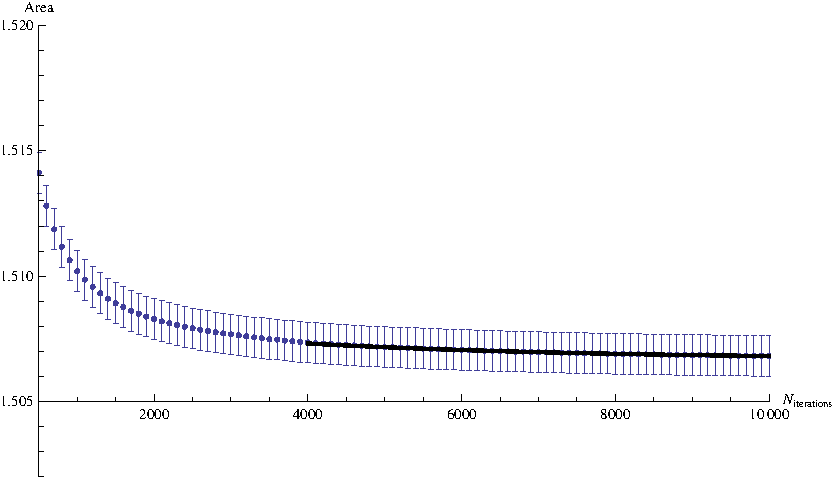
\includegraphics[scale=1.0]{fit_example.pdf}
  \caption{The mean area with error estimates as a function of the iteration $i$ obtained by using a random sampling method and $10^6$ samples. The thick black line  is obtained by fitting the exponential function A + B$\exp(\text{C} i)$ to the data.}
  \label{fig:fit_example}
\end{figure}

\noindent The function is fitted to the data using Mathematica, specifically the function NonLinearModelFit. One of the advantages of this function is that it takes the errors in the data into account when estimating the parameters and the error in the parameters of the function. If we let $i \rightarrow \infty$ the exponential term drops out (provided C is negative) and we obtain a value for the asymptote, equal to A. We can repeat this procedure for different sample sizes and different sample methods to obtain in every case a value for the parameter A and a corresponding value of the error of that parameter, taking into account the data errors.\\
\noindent Figure \ref{fig:asymptote_values} shown below gives the asymptote values for the different sample methods with uncertainty (again taking a confidence interval of 99$\%$) as a function of sample size. The black points correspond to random sampling, the red points to latin hypercube sampling and the blue points to orthogonal sampling. The horizontal line corresponds to the most accurately known values at the moment, $1.506 591 77$. To make the graph more clear the points are not placed at the exact same sample size, however the calculation itself was performed on the exact sample sizes mentioned above. One of the differences that is immediately seen is that the error is much smaller when the orthogonal method is used than in the other two cases. Also, the value of the orthogonal method is already accurate for small sample sizes while for orthogonal or latinhypercube sampling this is not the case.

\begin{figure}[H]
  \centering
  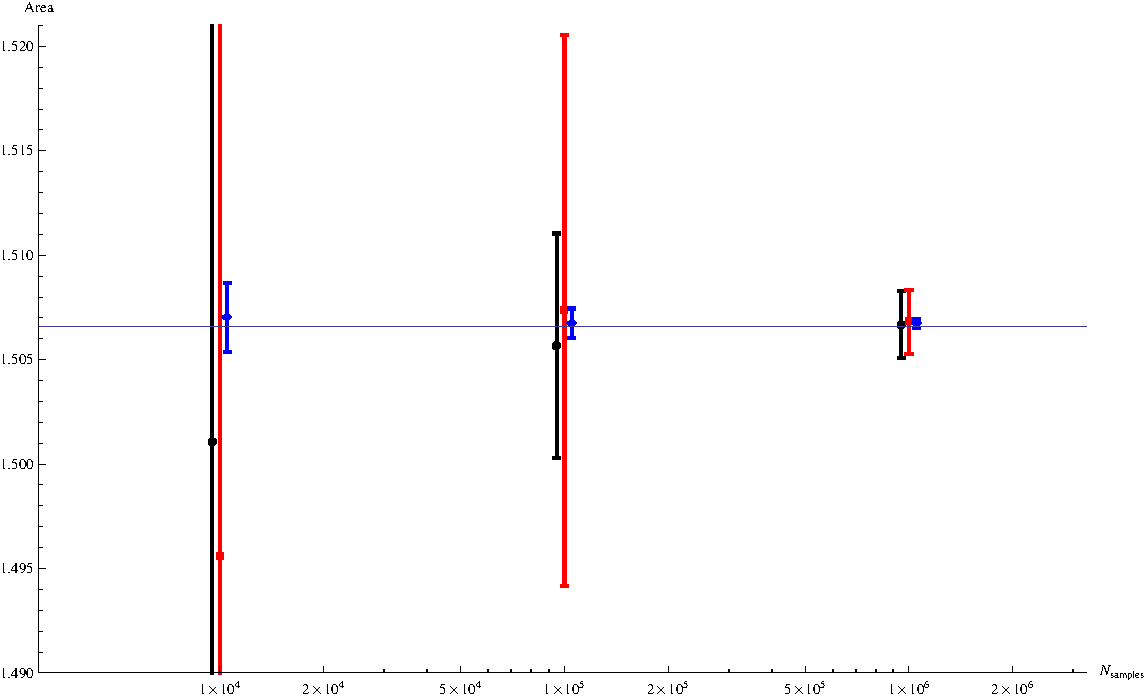
\includegraphics[scale=0.8]{asymptote_values.pdf}
  \caption{The asymptote values for different sample sizes and sampling methods. The black points correspond to random sampling, the red points to latinhypercube sampling and the blue points to orthogonal sampling.}
  \label{fig:asymptote_values}
\end{figure}

\noindent It is important to remark that the outcome of the asymptote values themselves are a stochastic variable, so by repeating the whole procedure one could obtain very different values for the asymptotes. Especially since we take $N_{\text{runs}} = 100$, repeating the whole procedure could give a very different outcome. However regardless of the specific asymptote values that are obtained, the error in the orthogonal method is much smaller than the error in the random sampling or latin hypercube sampling (this has been tested). Also using the orthogonal method the asymptote value approaces the best know value best. By the arguments above the orthogonal method will be used to estimate the area of the Mandelbrot set. The numerical values of the figure above for the orthogonal method are:\\
\newline
\begin{center}
\begin{table}[H]
\centering
\begin{tabular}{l c r}
Sample Size & Asymptote Value & Error\\
\hline
$10^4$ & 1.50703 & 0.00165 \\
$10^5$ & 1.50674 & 0.00071 \\
$10^6$ & 1.50673 & 0.00021 \\
\hline
\end{tabular}
\caption[width=5.0cm]{The asymptote values from figure \ref{fig:asymptote_values} for orthogonal sampling for different sample sizes including the error with a 99$\%$ confidence interval.}
\end{table}
\end{center}
So our final estimate for the area of the Mandelbrot set is $A_{\infty} = 1.50673 \pm 0.00021$. The best known value is within the confidence interval of 99$\%$ of this value.

\section{Discussion}

\noindent There are a few remarks to be made about this project. We used the method described in the section 'Methods' to calculate the asymptotic values. From experimenting with other values of $I_{\text{max}}$ it turns out that the accuracy with which one can get close to the best known value increases as the maximum number of iterations increases, which is expected, because the fit becomes more accurate. However, due to time limitations, we were only able to test this up to 10000 iterations, since we also need a significant number of samples and runs to get reasonable good statistics. \\
Secondly it is not clear from the documentation provided by Mathematica, what exactly the NonLinearModelFit does with the errors in the data to get an error in the parameter and hence in my case, the error for the asymptote. The error scales however with the square root of the number of points that are taken into account for the fit.\\
Thirdly, since I didn't use that many runs, calculating the asymptote values can differ greatly from one calculation to the next, since the asymptote value is a stochastic variable itself. For instance, it has happened that the asymptote value for $10^4$ samples and using random sampling gave almost exactly the same value as the best known value. However, as mentioned above, even though the asymptote was almost exactly right, the error remained very large, so there is a large spreading in area from one run to the next, but the mean ended up 'on accident' on the best known value.\\
Another remarkable issue I have found is that the difference between random sampling and latin hypercube sampling is not very large in terms of uncertainty in the final asymptote values. The method that is clearly much more precise is the orthogonal sampling. This error analysis was consistent en does not vary between experiments like the asymptote values themselves can.\\

\noindent In the model that I have used there is room for improvement. Firstly I was constrained by time and only having access to my own laptop for the computation. I had to balance between enough samples, enough runs for the statistics and large enough iterations to get a good final estimate. The combined running time of my program for all three sampling methods using $10^6$ samples, 100 runs and 10000 iterations was slightly less than an hour.\\
A possible improvement on the model is decreasing the area in which the samples are taken. Figure \ref{fig:mandelbrot} shows that there are large areas for which it is clear, for sufficiently high iteration level, that the area is inside or outside the Mandelbrot set. The sampling could be focused on the border area, using the same procedure as used above and then adding the area of the geometric shape that is not considered for sampling but is in the Mandelbrot set.

\begin{thebibliography}{2}
\bibitem{paper1} 
  http://www.mrob.com/pub/muency/pixelcounting.html
\bibitem{paper2}
  Ross, S.,\emph{Simulation}, 4th edition, 2006
\end{thebibliography}

\end{document}
